
\section{Application Study}
\label{sec:application study}

%A parallel application usually conforms to a combination of several basic communication patterns\cite{roth}. At its different execution phases, the application's communication behavior may follow different basic patterns respectively. \textcolor{blue}{When we look into the data flow during application execution, most parallel applications start with broadcast operation to distribute the data from root process to other processes\textcolor{red}{ref needed here}, followed by a series of computation and communication that conforms to certain pattern, which is usually the dominant part of application's execution. Before the application come to completion, all the working process will return their results to the root directly or hierarchically.} Parallel application's communication pattern usually involves lots of factors, such as communication intensity, operation-to-operation dependencies and the ``critical path" in its communication topology graph, etc. In this work, we focus on the locality of application's rank-to-rank communication topology graph.

A parallel application usually conforms to a combination of several basic communication patterns~\cite{roth}. 
At its different execution phases, 
the application's communication behavior may follow certain basic patterns respectively. 
There are many profiling tools available to capture 
information regarding communication patterns of parallel applications~\cite{tau,mpip,sst,oxbow}. 
They can provide information such as the percentage of different MPI operations, 
communication topology, the amount of data transferred between processes, etc.

There are many applications running on HPC systems such as Mira~\cite{bgq} and Titan~\cite{titan}. 
These applications are communication intensive and conform to various communication patterns. 
In this work, we select three representative applications from the DOE Design Forward Project. 
Each application exhibits a distinctive communication pattern that is commonly seen in HPC applications. 
We believe that the communication patterns of these applications 
are representative of a wide array of applications running on leadership-class machines. 
Specifically, we study the Algebraic MultiGrid Solver (AMG), 
Geometric MultiGrid (MultiGrid) and CrystalRouter MiniApps. 
The communication matrix presented in Figure~\ref{fig:apps_communication_matrix}
are generated with the IPM~\cite{ipm} data gathered from publicly available traces~\cite{designforwardwebpage}.

% MiniApps are reduced proxy applications that encapsulate the salient performance of larger full size applications \cite{miniapp}. Since we only focus on the dominant communication pattern of parallel applications, these MiniApps are perfect candidates for analysis the application's performance on different allocations or on new network architectures. We choose three MiniApps, namely, Algebraic Multigrid Solver(AMG), Geometric MultiGrid(MultiGrid) and CrystalRouter. Their representative communication patterns that are commonly seen in the HPC system workload. The communication pattern figures we present here are generated with the IPM \cite{ipm} data from \cite{designforwardwebpage}.


\begin{figure*}[htp]
    \centering
    \begin{subfigure}[t]{0.32\textwidth}
        \centering
        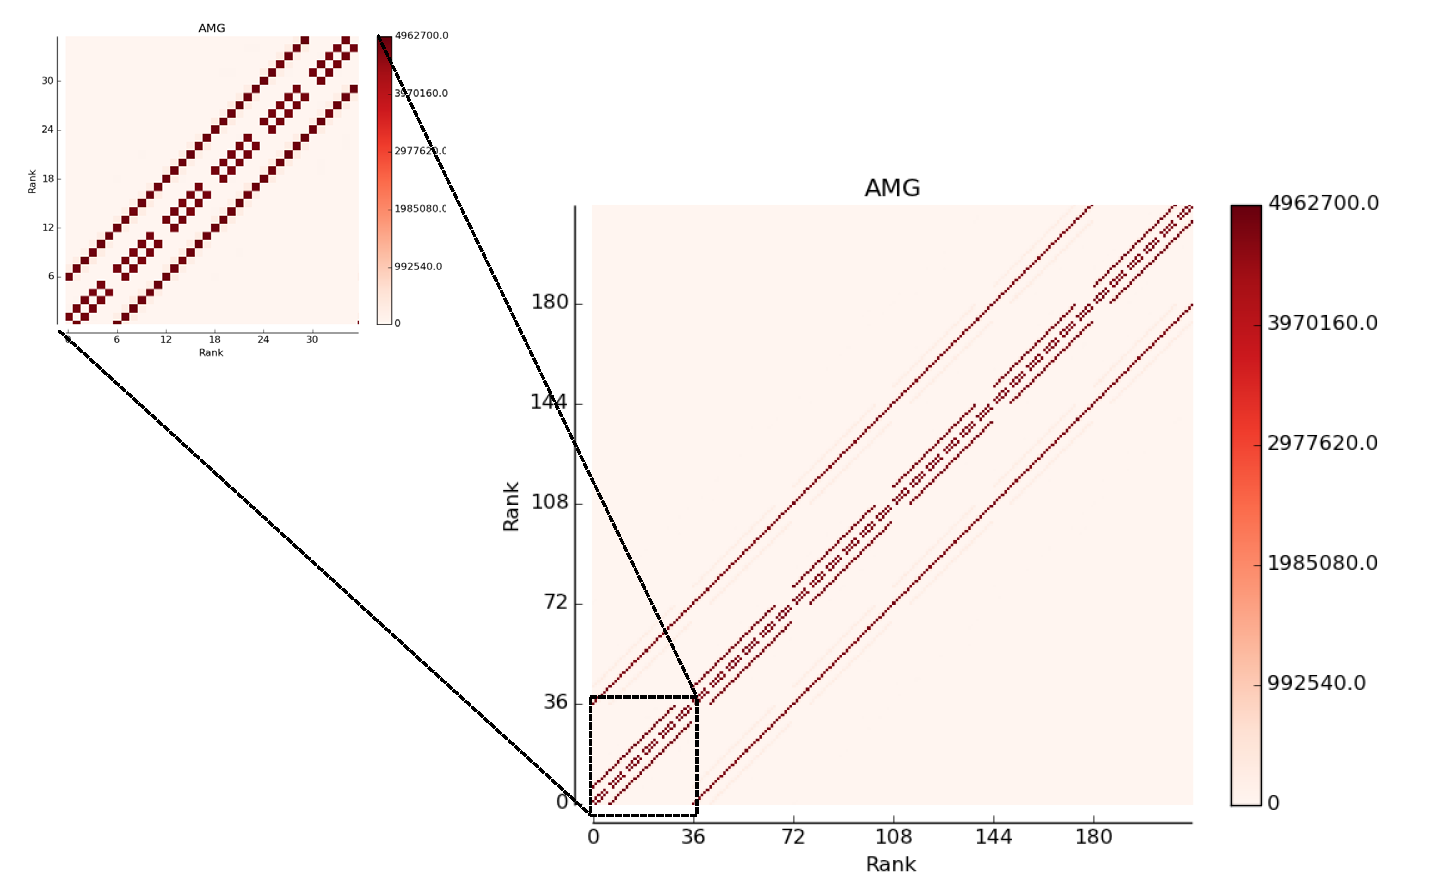
\includegraphics[height=1.5in]{figs/appstudy/amg/amg_pip}
        \caption{AMG}
        \label{fig:amg-communication-topology}
    \end{subfigure}
    \begin{subfigure}[t]{0.32\textwidth}
        \centering
        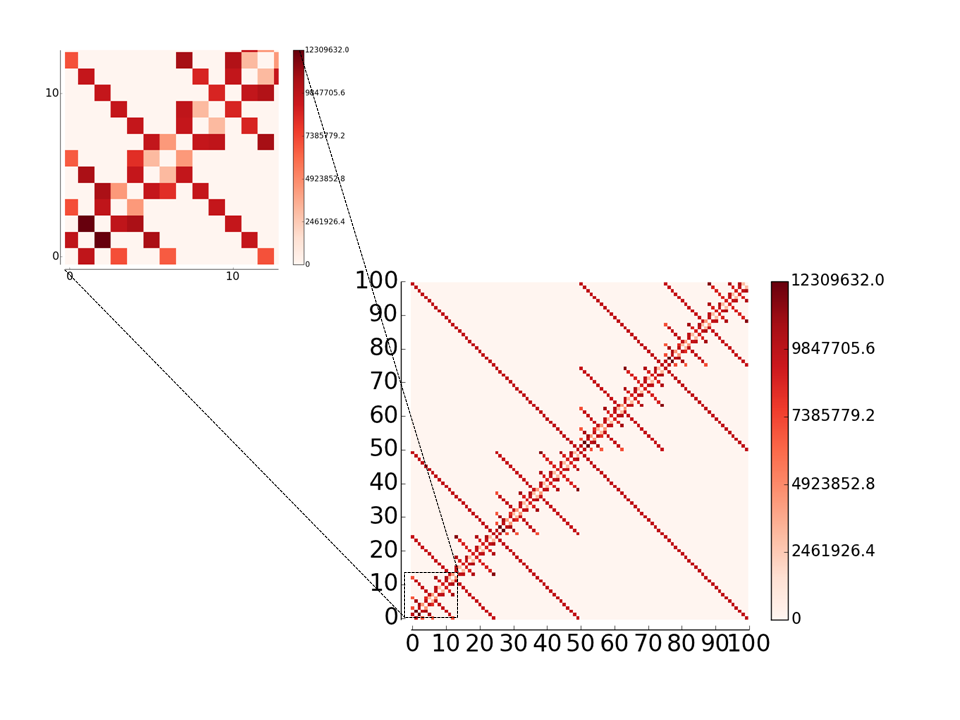
\includegraphics[height=1.5in]{figs/appstudy/cr/cr_pip}
        \caption{CrystalRouter}
        \label{fig:cr-communication-topology}
    \end{subfigure}
    \begin{subfigure}[t]{0.32\textwidth}
        \centering
        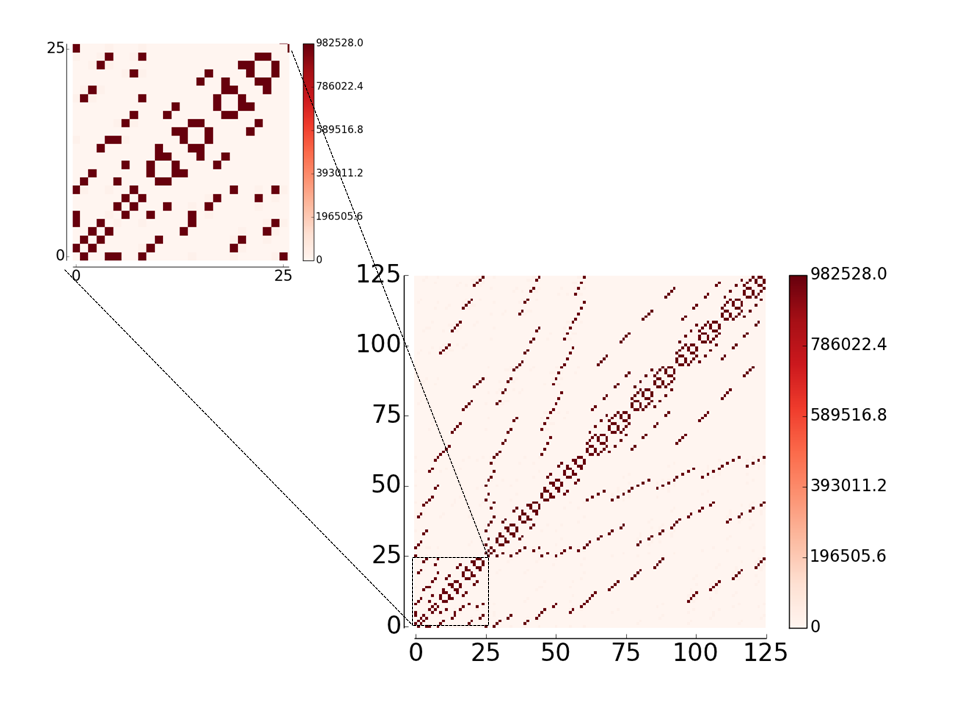
\includegraphics[height=1.5in]{figs/appstudy/mg/mg_pip}
        \caption{MultiGrid}
        \label{fig:mg-communication-topology}
    \end{subfigure}
    \caption{Applications rank-to-rank communication topology graph.}
    \label{fig:apps_communication_matrix}
\end{figure*}


\subsection{AMG}
\label{sec:amg}

%\begin{figure}[t!]
%    \centering
%    \begin{subfigure}[t]{0.25\textwidth}
%        \centering
%        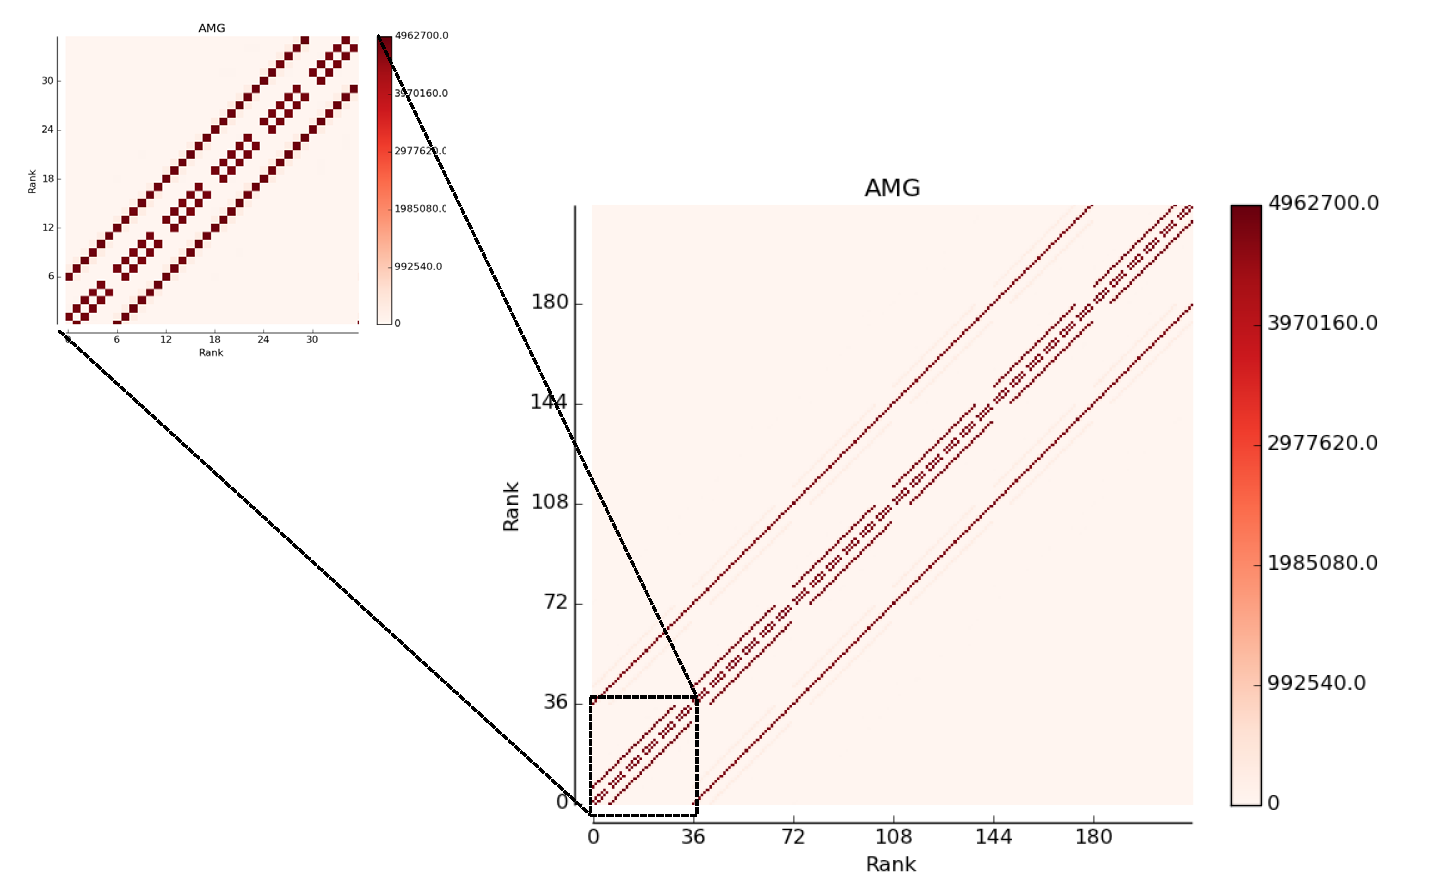
\includegraphics[height=1.5in]{figs/appstudy/amg/amg_pip}
%        \caption{}
%        \label{fig:amg-communication-topology}
%    \end{subfigure}%
%    ~
%    \begin{subfigure}[t]{0.24\textwidth}
%        \centering
%        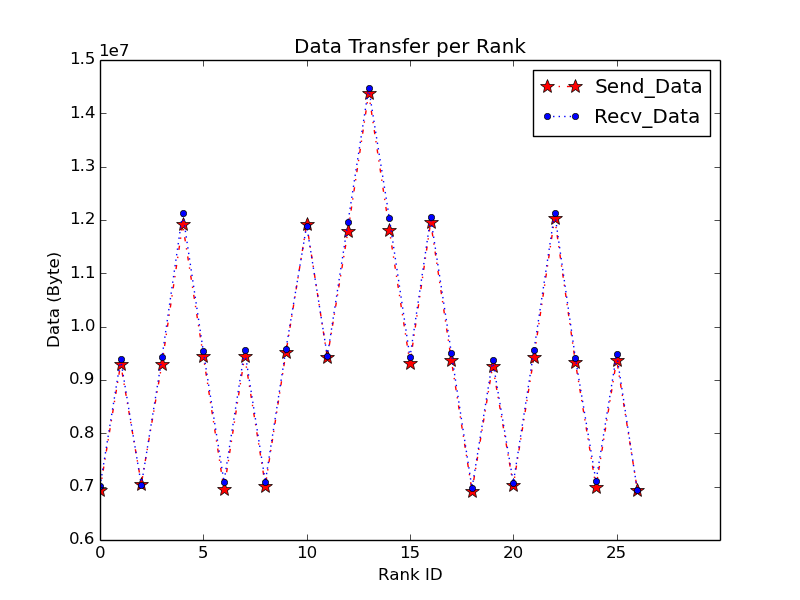
\includegraphics[height=1.2in]{figs/appstudy/amg/amg_data_transfer}
%        \caption{}
%        \label{fig:amg-data-trans}
%    \end{subfigure}
%    \caption{AMG. (a) Rank-to-rank communication topology graph, shows the intensity of communication between ranks in AMG. (b) The amount of data sent/received by each rank in AMG. Y-axis labels the amount of data transferred in MB, x-axis labels 216 ranks of AMG. }
%\end{figure}

The Algebraic MultiGrid Solver, or AMG, is a parallel algebraic multi-grid solver for linear systems arising from problems on unstructured mesh physics packages. It has been derived directly from the BoomerAMG solver that is being developed in the Center for Applied Scientific Computing (CASC) at LLNL \cite{amg}. The dominant communication pattern is regional communication with decreasing message size for different parts of the multi-grid v-cycle.

Figure~\ref{fig:amg-communication-topology} shows the communication topology of a small scale AMG execution with 216 MPI Ranks. Note that the dominant communication pattern of the application doesn't change with scale. We can make the observation that AMG's dominant communication pattern is 3D Nearest Neighbor, each rank has intensive communication with up to six neighbors, depending on the boundaries of the ranks. Applications with similar pattern include PARTISN \cite{partisn} and SNAP \cite{snap}.

%Figure~\ref{fig:amg-data-trans} shows the amount of data each rank transferred in the example execution. The data transferring of each rank is between 7MB to 16MB, corresponding to whether the rank is on a boundary or not.

\subsection{Crystal Router}
\label{sec:crystalrouter}

%\begin{figure}[t!]
%    \centering
%    \begin{subfigure}[t]{0.25\textwidth}
%        \centering
%        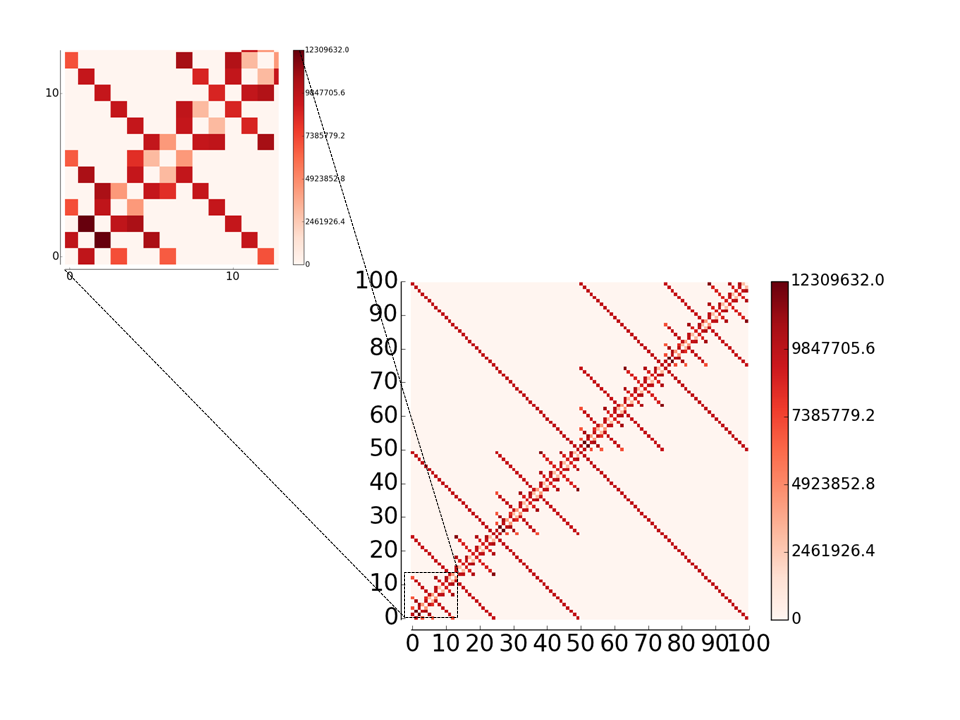
\includegraphics[height=1.5in]{figs/appstudy/cr/cr_pip}
%        \caption{Communication Topology}
%        \label{fig:cr-communication-topology}
%    \end{subfigure}
%    ~
%    \begin{subfigure}[t]{0.22\textwidth}
%        \centering
%        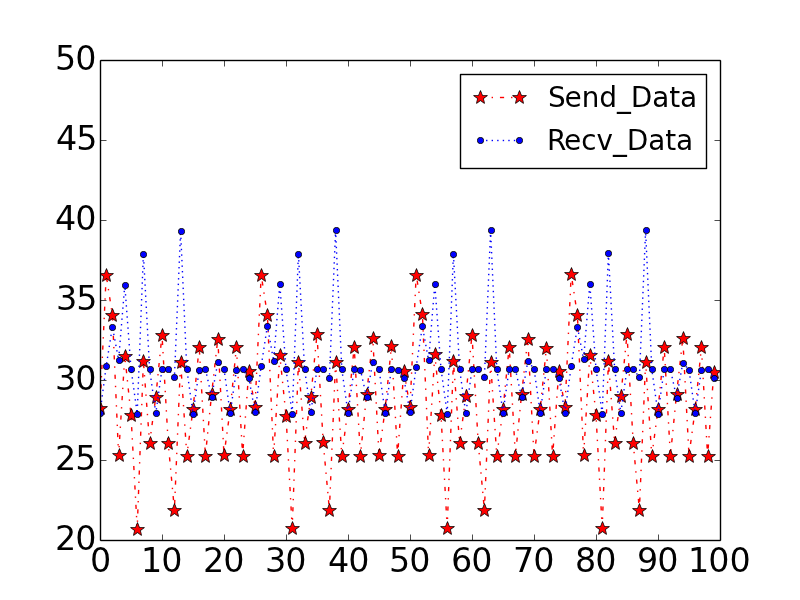
\includegraphics[height=1.2in]{figs/appstudy/cr/cr_data_transfer}
%        \caption{Data Volume}
%        \label{fig:cr-data-trans}
%    \end{subfigure}
%    \caption{CrystalRouter. (a) Rank-to-rank communication topology graph, shows the intensity of communication between ranks in CrystalRouter. (b) The amount of data sent/received by each rank in CrystalRouter. Y-axis labels the amount of data transferred in MB, x-axis labels 100 ranks of CrystalRouter. }
%\end{figure}

The second MiniApp covered is CrystalRouter, the extracted communication kernel of the full application Nek5000~\cite{crystalrouter}, which is a spectral element CFD application developed at Argonne National Laboratory \cite{nek5000}. It features spectral element multi-grid solvers coupled with a highly scalable, parallel coarse-grid solver that is widely used for projects including ocean current modeling, thermal hydraulics of reactor cores, and spatiotemporal chaos. CrystalRouter demonstrates the ``many-to-many'' communication pattern through a scalable multi-stage communication process. The way CrystalRouter works is nodes compute for a while, then synchronize and communicate, continually alternating between these two types of activities.

The collective communication in CrystalRouter utilizes a recursive doubling approach. Ranks in CrystalRouter conform to a $n$-dimensional hypercube and recursively split into ($n$-1)-dimensional hypercubes, with communication occurring along the splitting plane. The pattern of this communication can be found in Figure~\ref{fig:cr-communication-topology}. By nature of the logarithmic splitting process, a substantial portion of the communication occurs in small neighborhoods of ranks. CrystalRouter represents a group of applications whose dominant communication is a hybrid of multi-stage local and hierarchical global communication, and shares similarities with most MPI collective communication implementations.

%Figure~\ref{fig:cr-data-trans} shows the amount of data each rank transferred in CrystalRouter, which ranges between 20MB to 36MB. This is due to the rank counts not matching one-for-one with points in the hypercube.

\subsection{MultiGrid}
\label{sec:multigrid}

%\begin{figure}[t!]
%    \centering
%    \begin{subfigure}[t]{0.25\textwidth}
%        \centering
%        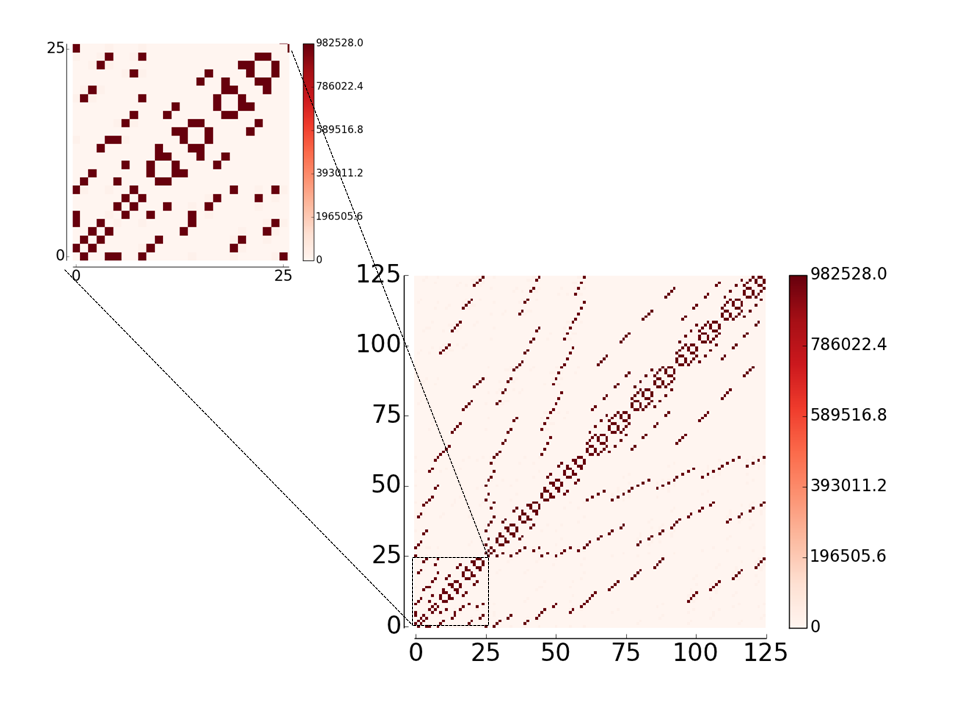
\includegraphics[height=1.5in]{figs/appstudy/mg/mg_pip}
%        \caption{Communication Topology}
%        \label{fig:mg-communication-topology}
%    \end{subfigure}
%    ~
%    \begin{subfigure}[t]{0.22\textwidth}
%        \centering
%        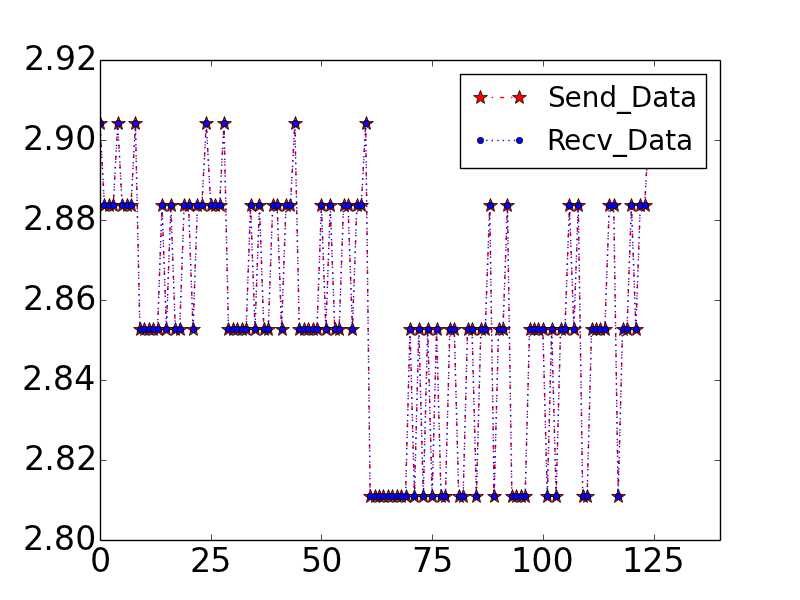
\includegraphics[height=1.2in]{figs/appstudy/mg/mg_data_transfer}
%        \caption{Data Volume}
%        \label{fig:mg-data-trans}
%    \end{subfigure}
%    \caption{MultiGrid. (a) Rank-to-rank communication topology graph, shows the intensity of communication between ranks in MultiGrid. (b) The amount of data sent/received by each rank in MultiGrid. Y-axis labels the amount of data transferred in MB, x-axis label 125 ranks of MultiGrid. }
%\end{figure}

MultiGrid is geometric multi-grid v-cycle from the production elliptic solver BoxLib, a software framework for massively parallel block-structured adaptive mesh refinement (AMR) codes \cite{boxlib}. MultiGrid conforms to many-to-many communication pattern with decreasing message size and collectives for different parts of the multi-grid v-cycle. It is widely used for structured grid physics packages. 

Figure~\ref{fig:mg-communication-topology} shows the communication topology of MultiGrid with 125 ranks. We can see intensive communication along the diagonal that resembles nearest neighbor communication, similar to AMG. However, the communication topology leads to a greater ``spread'' of communication across the set of ranks, challenging the maximization of communication locality with respect to rank. In this sense, it can be considered a ``many-to-many'' pattern. Applications with such similar dominant communication pattern are like FillBoundary, another PDE solver code in \cite{boxlib}.

%Figure~\ref{fig:mg-data-trans} shows the amount of data transferred between ranks in MultiGrid. For this miniapp, The data transferred per rank is relatively small and stable, between 2.8MB to 2.9MB.



